
\textbf{PUT the examples right in the place where it is mentioned in the theory.!} 
"As we have seen in section 2.1.1.... and in section 2.2.2......"

In this first analysis, we rely on 

This analysis relies on \texttt{1inter\_stationary.R} code from the \textbf{/Scripts-R/} folder of the github repository.



The block-length selection an important issue of the analysis. It is important to choose a block-length which is large enough for the limiting arguments supporting the GEV approximation (see (\ref{exttheom})) to be valid, either a large bias in the estimates could occur. For example, if this is too short, the maxima may be too close of each other to assume independence. But a large block-length implies less data to work with, and thus a large variance of the estimates. A compromise must be found between bias and variance and as pointed out in \hyperref[sec::1]{chapter \textbf{\ref{sec::1}}}, yearly blocks seem justifiable not only for this reason (difficult to study?) but especially for their interpretability and ease of use.

\addcontentsline{toc}{subsection}{R packages for EVT}
\subsubsection*{R packages in EVT}

A plenty of packages exist for modelling extreme values in R. We have explored most of them and we used some to do the following analysis. We made comparisons and the results are the same for similar methods. Regarding the classic EVT analysis, we must name the following : 
\vspace*{-.2cm}
\begin{itemize}
\item[$\blacktriangleright$] \textbf{\texttt{ismev, evd, extRemes}} (good for a wide nonstationary analysis with POT and nice tutorials, see e.g. \citet{gilleland_extremes_2016})  \texttt{, \textbf{POT}} (see \citet{ribatet_users_2006})\texttt{, \textbf{evir},} \texttt{\textbf{fExtremes}}, $\dots$
\end{itemize}

Whereas lots of the package are doing the same analysis but with different tools, we decided to rely mostly on \texttt{ismev} as it is the package used in the book of \citet{coles_introduction_2001}.

\section{Estimation of the Model}

Whereas the whole content of chapter \hyperref[sec::1]{\textbf{\ref{sec::1}}} is important to understand the concepts used in this section, we will now be mostly based on inferential methods discussed in \hyperref[sec::gevinfernce]{section\textbf{ \ref{sec::gevinfernce}}}

\subsection{Maximum Likelihood}\label{sec:mlepratic}

Relying on the R packages cited above ,but also by checking it manually, i.e. by numerically solving the optimization problem, that is minimizing the negative log-likelihood, with the \texttt{nlm} routine using a Newton-Raphson algorithm (originated from \citet{dennis_numerical_1987}). This is based on approximating the log-likelihood by a quadratic function, the second order Taylor series approximation of the log-likelihood for a given point.  The results are shown in table \ref{tab:estlik} :
\vspace{-.3cm}
\begin{table}[!htbp] \centering 
  \caption{shows the maximum likelihood estimation of the three GEV parameters} 
  \label{tab:estlik} 
\begin{tabular}{@{\extracolsep{5pt}} cccc} 
\\[-1.8ex]\hline 
\hline  \\[-1.8ex] 
 & Location $\mu$ & Scale $\sigma$ & Shape $\xi$ \\ 
\hline \\[-1.8ex] 
Estimates (s.e.) & $30.587$ ($0.216$)& $2.081$ ($0.155$) & $\boldsymbol{-0.254}$ ($0.067$) \\ 
\hline \\[-1.8ex] 
\end{tabular} 
\end{table} 
\vspace{-.3cm}

From this table \ref{tab:estlik}, an important thing to note is the value of the \textbf{shape} parameter which is negative which means that we are under a Weibull-type distribution  From figure \ref{gev3plot} this means that the density distribution has the form of the red line, i.e. having a .
Moreover, we confirmed that by doing a likelihood ratio test comparing this distribution with a Gumbel distribution. We obtained a p-value of $10^{-3}$ leading to a rejection of the Gumbel hypothesis. This obviously implies rejection of the Fréchet distribution.

The Weibull-type implies that the distribution have an estimated right endpoint given by $\hat{x}_*=\hat{\mu}-\hat{\sigma}\cdot\hat{\xi}^{-1}=38.77$. Comparing this value with the maximum value of the series (=36.6) tells us that the sample properties of this model take into account the uncertainty, from the fact that there are only 116 years of data. Hence, it allows to go beyond this maximum value, with very small probability. This is also highlighted in figure \ref{fig:rl_empdes} (right plot) where we remark that there are still probabiliy mass beyond the minimum and the maximum values of the series.

The \textbf{profile} log-likelihood intervals for the parameters are shown in figure \ref{fig:proflikpar} in \hyperref[app:fig]{appendix \ref{app:fig}}, provided by the \texttt{ismev} package. These intervals are constructed in the following way : Search for the horizontal line Substracting the maximum log-likelihood $\ell$ half the corresponding upper quantile of the $\chi^2_{\text{df}}$ for the $\text{df}=1$ parameter of interest. We notice that :
\begin{itemize}
\item Even at $99\%$, the interval for $\hat{\xi}$ does not contain 0 supporting our statement that the distribution is left heavy-tailed and right bounded.
\item The intervals do not present much asymetries. In fact, this will be more relevant for return levels as we will see in section
\end{itemize}


\subsection{Other Methods}


\section{Diagnostics}

\begin{figure}[!htb]
\centering	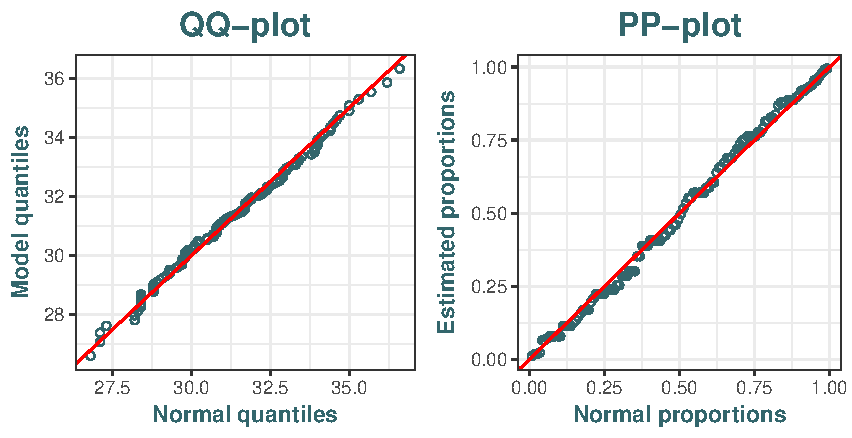
\includegraphics[width=.7\linewidth]{pp_qqplot.pdf}\caption{}\label{fig:ppqqplot}
\end{figure}


\section{Return Levels}

Explore why the return leels go beyond the right endpoint of the distribution (when $\xi<0$ as here), for which return period, etC...

\begin{figure}[!htb]
\centering	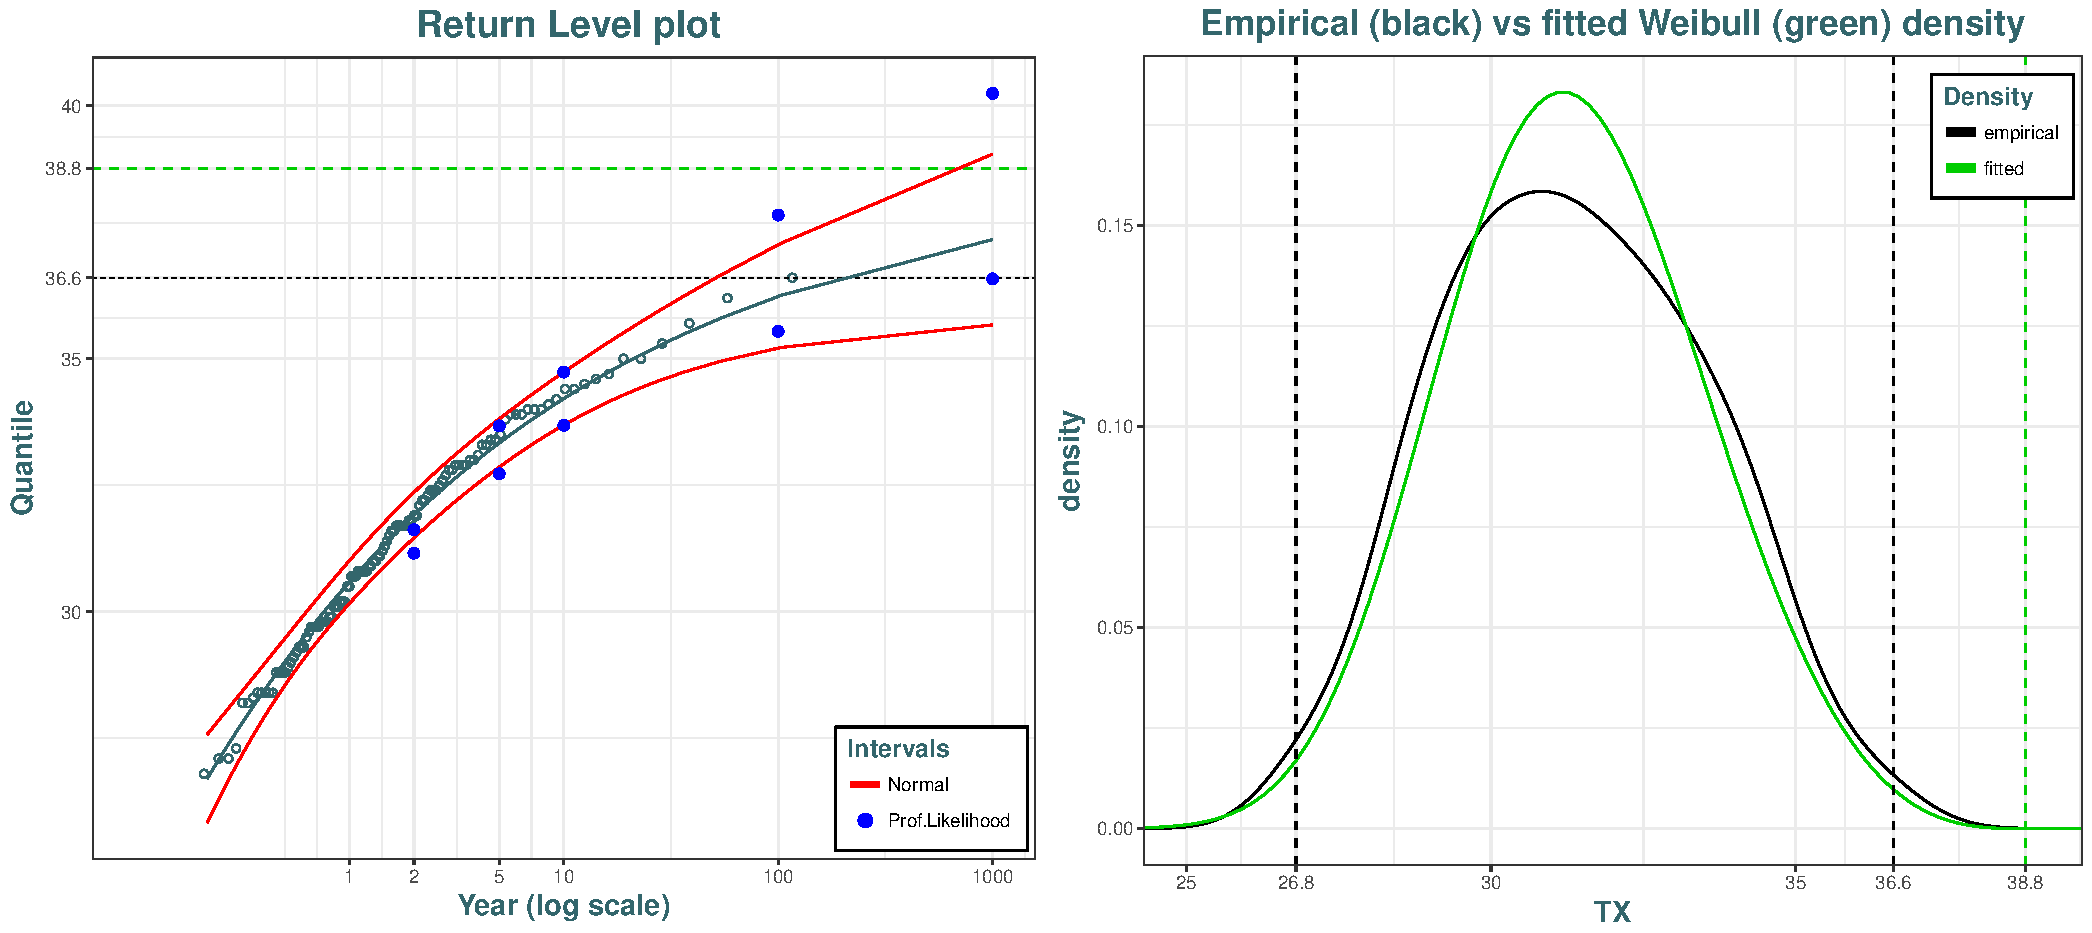
\includegraphics[width=.75\linewidth]{rl_empdes.pdf}\caption{ The left and right vertical dotted lines represent respectively the minimum and the maximum value of the yearly maxima series.}\label{fig:rl_empdes}
\end{figure}


\subsection{Profile Likelihood}



\section{Comments and Comparisons with POT}
